In this chapter I will present the results obtained for Q-dots with 2 to 6 electrons.
In order to find the optimal parameters I proceeded as follows:
\begin{enumerate}
  \item Produce a plot of the function $E(\bm{\alpha})$ to see how it behaves,
  \item starting from a resonable value looking at the plot, use DFP minimization to find the optimal parameters.
\end{enumerate}
The uncertainties are calculated through \autoref{staterror} assuming no statistical correlation (see \autoref{correlation}).

\section{Simple Minimization with graphics}

The first thing I did was to calculate the energy in a range of possible values for the variational parameters to make graphics and see how the energy behaves in the parameters space.
The values are calculated 9 at the time, thanks to the reweighing technique (\autoref{reweight}), using the central values to sample the configurations as shown in \autoref{RewVarPlot}.
Doing this we are able to reduce the computation time of about $70\%$.
Since we are only interested in understanding the qualitative behaviour of the energy respect to the parameters, to make this plots we use just $10^6$ Monte Carlo cycles for each configuration.
I noticed that the computation time goes like $\sim\frac{N^2}{4}$, meaning that the algorithm is adequately optimized and it could handle bigger systems as well.

\begin{figure}[h]
  \centering
  \includegraphics[width=.5\textwidth]{Schemes/sampling.pdf}
  \caption{Reweighing methods producing $E(\bm{\alpha})$ plots.}
  \label{RewVarPlot}
\end{figure}

In \autoref{varplot} are shown the plots of the energy for $N=2,\>3,\>5$ and $6$ electrons.
For generating these graphics I varied the parameters through $21$ values for $a$ and $21$ for $b$.
As we can see the surface has a strong valley shape, meaning that there is a direction along which it is harder to find the exact minimum.
Anyway this is not a big problem since in that direction, around the minimum the energy variations are comparable with our uncertainties.
Orienting the $a$ or $b$ axis to be perpendicular to the sheet we can already try to extrapolate the optimal parameters and the minimized energy as presented in \autoref{varplot2ab} for the 2-electrons case.
In \autoref{VarPlotMinima} are presented the minimum registered energy values of the plots together with the corresponding parameters for $N=2,\>3,\>5$ and $6$.

\begin{table}[H]
  \centering
  \begin{tabular}{c|c|c|c}
    \toprule
    $N$ & $E_{min}\>[H*]$ & $a$ & $b$ \\
    \hline
    $2$ & $3.0001(2)$ & $0.820$ & $0.275$ \\
    $3$ & $6.3757(4)$ & $0.98$ & $0.50$ \\
    $5$ & $14.9947(7)$ & $0.94$ & $0.56$ \\
    $6$ & $20.2073(8)$ & $0.98$ & $0.60$ \\
    \bottomrule
  \end{tabular}
  \caption[Energy minima and correspondent parameters for $N=2,\>3,\>5,\>6$ calculated by manually varying the parameters.]{Energy minima and correspondent parameters for $N=2,\>3,\>5,\>6$ calculated by manually varying the parameters. In parentheses are the uncertainties in the last digit. All values are for $\omega=1$}
  \label{VarPlotMinima}
\end{table}

\begin{figure}[h]
  \begin{minipage}{0.5\textwidth}
    \centering
    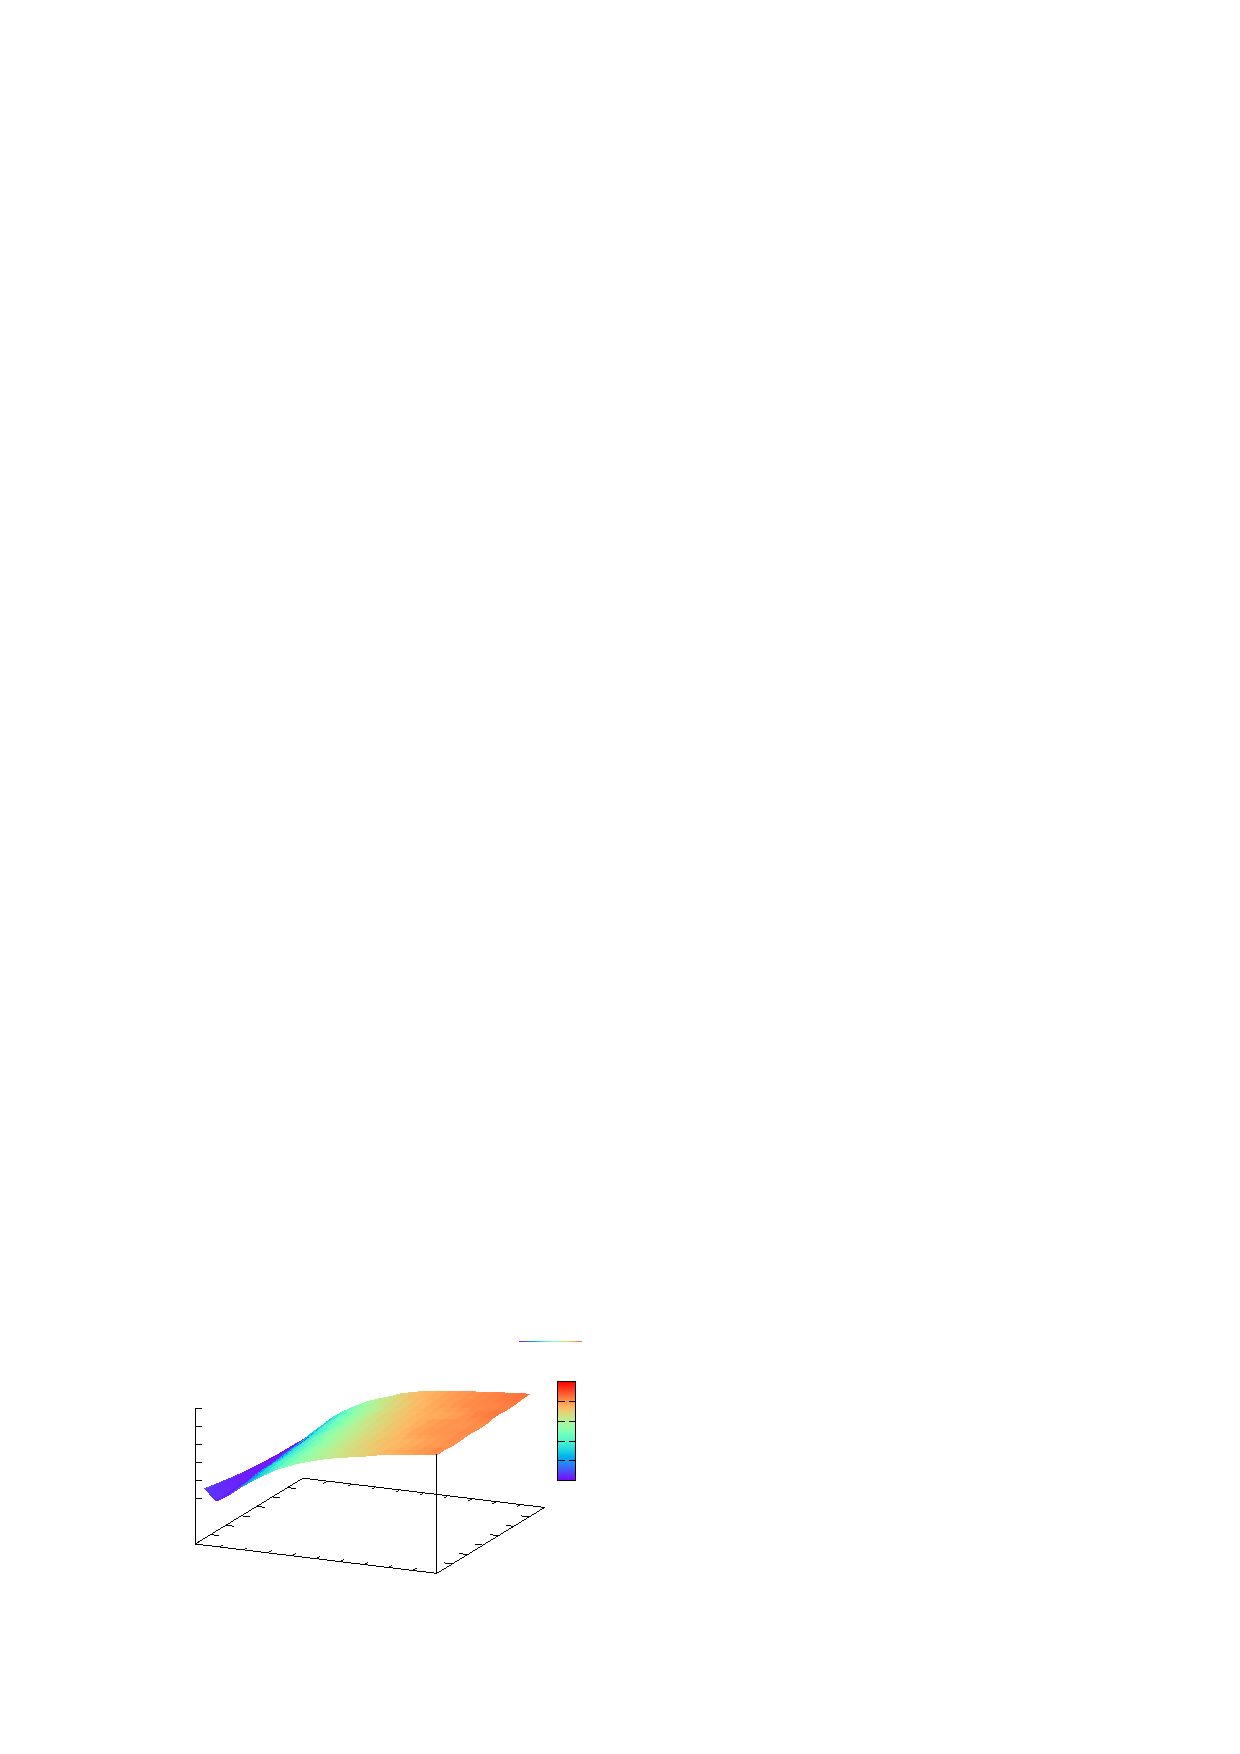
\includegraphics[width=\textwidth]{Graphics/surf2.pdf}
    \includegraphics[width=\textwidth]{Graphics/surf5.pdf}
  \end{minipage}
  \begin{minipage}{0.5\textwidth}
    \centering
    \includegraphics[width=\textwidth]{Graphics/surf3.pdf}
    \includegraphics[width=\textwidth]{Graphics/surf6.pdf}
  \end{minipage}
  \begin{center}
    \caption{Energy plots for $N=2,\>3,\>5,\>6$.}
    \label{varplot}
  \end{center}
\end{figure}

\begin{figure}[h]
  \centering
  \includegraphics[width=\textwidth]{Graphics/surf2ab.pdf}
  \caption{Energy plot for N=2. Lateral views.}
  \label{varplot2ab}
\end{figure}

\subsection{$N=4$ and Hund's rules}

The results for the three configurations for the 4-particle Quantum dot are presented in \autoref{VarPlotMinima4} and \autoref{varplot4}.
We notice that the ground state is given by $L=0$ and $S=1$ in agreement with the Hund's first rule, which states that for a given electron configuration the term with the maximum multiplicity has the lowest energy.

The Hund's first rule has been seen to be followed by Q-dots also in paper like Refs\cite{Pederiva2000,Harju1999} and experimentally in Refs\cite{Kouwenhoven1997,Tarucha1996}.
The second Hund's rules, for which at a given multiplicity the lowest energy is given by the highest angular momentum, is not seen to be valid for Q-dots.

\begin{table}[H]
  \centering
  \begin{tabular}{c|c|c|c|c}
    \toprule
    $L$ & $S$ & $E_{min}\>[H*]$ & $a$ & $b$ \\
    \hline
    $0$ & $1$ & $10.2892(5)$ & $0.96$ & $0.58$ \\
    $0$ & $0$ & $10.351(2)$ & $1.18$ & $0.7$ \\
    $2$ & $0$ & $10.4878(6)$ & $1.04$ & $0.58$ \\
    \bottomrule
  \end{tabular}
  \caption[Energy minima and correspondent parameters for $N=4$ calculated by manually varying the parameters.]{Energy minima and correspondent parameters for $N=4$ calculated by manually varying the parameters. In parentheses are the uncertainties in the last digit. All values are for $\omega=1$.}
  \label{VarPlotMinima4}
\end{table}

\begin{figure}[h]
  \begin{minipage}{0.5\textwidth}
    \centering
    \includegraphics[width=\textwidth]{Graphics/surf401.pdf}
  \end{minipage}
  \begin{minipage}{0.5\textwidth}
    \centering
    \includegraphics[width=\textwidth]{Graphics/surf400.pdf}
  \end{minipage}
  \begin{center}
    \includegraphics[width=.5\textwidth]{Graphics/surf420.pdf}
    \caption{Energy plots for $N=4$ in all the possible configurations of $L$ and $S$.}
    \label{varplot4}
  \end{center}
\end{figure}

\section{DFP minimization}
Calculations with the Davidon-Fletcher-Powell algorithm were challenging because of the flatness about the minimum of the Energy.
I used a step of $0.0001$ for calculating derivates and $5\times10^7$ Monte Carlo cycles for each energy calculation.
The computation of the minimum stops either when the gradient satisfies the threshold $\norm{\nabla E(\bm{\alpha})}\leq0.001$ or when the Newton's algorithm for the line search stops working because derivatives become too small compared with the statistical fluctuations of the energy.
In order to achieve more accuracy I would needed to use more MC-cycles and calculation would have been unsustainable for the computational power and the time at my disposal.

\begin{table}[H]
  \centering
  \begin{tabular}{c|c|c|c|c|c}
    \toprule
    $N$ & $L$ & $S$ & $E_{min}\>[H*]$ & $a$ & $b$ \\
    \hline
    $2$ & $0$ & $0$ & $3.00013(2)$ & $0.87893$ & $0.31450$ \\
    $3$ & $1$ & $1/2$ & $6.37632(6)$ & $1.03177$ & $0.55051$ \\
    $4$ & $0$ & $1$ & $10.28932(7)$ & $0.95629$ & $0.57807$ \\
    $4$ & $0$ & $0$ & $10.35134(7)$ & $1.00507$ & $0.58889$ \\
    $4$ & $2$ & $0$ & $10.48903(9)$ & $1.02226$ & $0.56605$ \\
    $5$ & $1$ & $1/2$ & $14.99571(9)$ & $0.97274$ & $0.58759$ \\
    $6$ & $0$ & $0$ & $20.2086(1)$ & $0.992936$ & $0.611292$ \\
    \bottomrule
  \end{tabular}
  \caption[Energy minima and correspondent parameters calculated with DFP.]{Energy minima and correspondent parameters calculated with DFP. In parentheses are the uncertainties in the last digit. All values are for $\omega=1$.}
  \label{DFPMinima}
\end{table}

The values are close to those estimated with manually plotting the energy but uncertainties are $\sim 10$ times less.
The minimized parameters also changed and this is certainly due to the high uncertainties of the energies in the plots, but also to the flatness about the minima that makes difficult finding exact parameters.
In \autoref{contour} are shown the iterations that took the algorithm to reach the minimum for the case $N=2$. % TODO comments
The first iteration went along the steepest descent direction, while the next iteration was pointing already right about the minima.
The small steps after the change in direction are made in order to find a point with positive second derivative because using the Newton's method with a negative second derivative would lead to a maximum rather than a minimum.

\begin{figure}[h]
  \centering
  \includegraphics[width=\textwidth]{Graphics/contour2.pdf}
  \caption{Path of the DFP minimization for $N=2$.}
  \label{contour}
\end{figure}

\section{Validation}

Comparisons between results of different work are not easy because of the different values used for $\epsilon$ and $\omega$.
The only works I found to have those values as mine are Ref\cite{larsevind} with variational Monte Carlo and Ref\cite{PedersenLohne2011} with diffusion Monte Carlo, but they made calculation only for closed shell Quantum dots, namely $N=2$ and $N=6$.
Their results, together with mine, are shown in \autoref{comparisons}.
The difference between the results is mainly due to the different trial wave functions used and the method.
In particular we notice smaller values for the diffusion Monte Carlo technique.
Anyway this comparison is good to validate the rightness of my results.

\begin{table}[H]
  \centering
  \begin{tabular}{c|c|c}
    \toprule
    $E$ & $E_{VMC}$ & $E_{DMC}$ \\
    \hline
    $3.00013(2)$ & $3.00029(3)$ & $3.00000(3)$ \\
    $20.2086(1)$ & $20.1899(2)$ & $20.1597(2)$ \\
    \bottomrule
  \end{tabular}
  \caption[Comparison of our results with those in Ref\cite{larsevind} and Ref\cite{PedersenLohne2011} for closed shell Q-dots.]{Comparison of our results ($E$) with those in Ref\cite{larsevind} ($E_{VMC}$) and Ref\cite{PedersenLohne2011} ($E_{DMC}$) for closed shell Q-dots. In parentheses are the uncertainties in the last digit. All values are for $\omega=1$.}
  \label{comparisons}
\end{table}
